code
Latex
download
content_copy
expand_less
\documentclass{article}
\usepackage{amsmath}
\usepackage{amssymb}
\usepackage{graphicx}
\usepackage{tikz}
\usepackage{pgfplots}
\pgfplotsset{compat=1.18}
\usepackage{booktabs}
\usepackage{xcolor}

% Custom Environments
\newenvironment{lesson-meta}{}{}
\newenvironment{item-analysis}{}{}
\newenvironment{model-discuss}{}{}
\newenvironment{concept-box}{}{}
\newenvironment{concept-summary}{}{}
\newenvironment{example}[1]{\textbf{Example #1}\par}{\par}
\newenvironment{tryit}[1]{\textbf{Try It! #1}\par}{\par}
\newenvironment{practice}[2]{\textbf{#1}\quad}{\par}
\newenvironment{te-addendum}[2]{}{}

% Custom Commands
\newcommand{\answer}[1]{}
\newcommand{\placeholder}[2]{[\textit{#1: #2}]}
\newcommand{\uncertain}[2]{#1}
\newcommand{\te}[1]{}

\begin{document}

\begin{lesson-meta}
\textbf{4-4 Adding and Subtracting Rational Expressions} \\
\textbf{I CAN...} find the sum or difference of rational expressions. \\
\textbf{VOCABULARY} compound fraction \\
\textbf{ESSENTIAL QUESTION} How do you rewrite rational expressions to find sums and differences?
\end{lesson-meta}

\begin{model-discuss}
\textbf{CRITIQUE \& EXPLAIN}
Teo and Evander find the following exercise in their homework:
\[ \frac{1}{2} + \frac{1}{3} + \frac{1}{9} \]

\placeholder{photo}{A tablet displaying the math problem 1/2 + 1/3 + 1/9}

\begin{enumerate}
    \item[\textbf{A.}] Teo claims that a common denominator of the sum is $2 + 3 + 9 = 14$. Evander claims that it is $2 \cdot 3 \cdot 9 = 54$. Is either student correct? Explain why or why not.
    \item[\textbf{B.}] Find the sum, explaining the method you use.
    \item[\textbf{C.}] \textbf{Construct Arguments} Timothy states that the quickest way to find the sum of any two fractions with unlike denominators is to multiply their denominators to find a common denominator, and then rewrite each fraction with that denominator. Do you agree?
\end{enumerate}
\end{model-discuss}

\begin{example}{1}
\textbf{Add Rational Expressions With Like Denominators}

\textbf{What is the sum?}

\textbf{A.} $\frac{x}{x + 4} + \frac{5}{x + 4}$

\textit{Note: When denominators are the same, add the numerator.}
\[ = \frac{x + 5}{x + 4} \]
The sum $\frac{x}{x + 4} + \frac{5}{x + 4}$ is $\frac{x + 5}{x + 4}$.

\textbf{B.} $\frac{2x + 1}{x^2 + 3x} + \frac{3x - 8}{x(x + 3)}$

\textit{Note: Multiply the factors in the denominator. $x(x + 3) = x^2 + 3x$. The denominators are the same, so the numerators may be added.}
\begin{align*}
    &= \frac{(2x + 1) + (3x - 8)}{x^2 + 3x} \\
    &= \frac{(2x + 3x) + (1 - 8)}{x^2 + 3x} \\
    &= \frac{5x - 7}{x^2 + 3x}
\end{align*}
The sum $\frac{2x + 1}{x^2 + 3x} + \frac{3x - 8}{x(x + 3)}$ is $\frac{5x - 7}{x^2 + 3x}$.
\end{example}

\begin{concept-box}
\textbf{USE STRUCTURE}
Compare addition of numerical and algebraic fractions:
$\frac{1}{5} + \frac{3}{5} = \frac{1 + 3}{5} = \frac{4}{5}$
In the same way,
$\frac{x}{x + 4} + \frac{5}{x + 4} = \frac{x + 5}{x + 4}$.
\end{concept-box}

\begin{tryit}{1}
Find the sum.
\begin{enumerate}
    \item[\textbf{a.}] $\frac{10x - 5}{2x + 3} + \frac{8 - 4x}{2x + 3}$
    \item[\textbf{b.}] $\frac{x - 5}{x + 5} + \frac{3x - 21}{x + 5}$
\end{enumerate}
\end{tryit}

\begin{example}{2}
\textbf{Identify the Least Common Multiple of Polynomials}

\textbf{How can you find the least common multiple (LCM) of polynomials?}

\textbf{A.} $(x + 2)^2$, $x^2 + 5x + 6$
Factor each polynomial.
$(x + 2)^2 = (x + 2)(x + 2)$
$x^2 + 5x + 6 = (x + 2)(x + 3)$
The LCM is the product of the factors. Include the greatest number of any one factor in each polynomial.
LCM: $(x + 2)(x + 2)(x + 3)$ or $(x + 2)^2(x + 3)$

\textbf{B.} $x^3 - 9x$, $x^2 - 2x - 15$, $x^2 - 5x$
Factor each polynomial.
$x^3 - 9x = x(x^2 - 9) = x(x + 3)(x - 3)$
$x^2 - 2x - 15 = (x + 3)(x - 5)$
$x^2 - 5x = x(x - 5)$
LCM: $x(x + 3)(x - 3)(x - 5)$

\textit{Note: Each distinct polynomial becomes a factor of the LCM. Using the LCM can mean less work later.}
\end{example}

\begin{concept-box}
\textbf{USE STRUCTURE}
The LCM of 6 and 15 is 30, not 90. $\frac{1}{6} + \frac{1}{15} = \frac{1}{2 \cdot 3} + \frac{1}{3 \cdot 5} = \frac{1 \cdot 5 + 1 \cdot 2}{2 \cdot 3 \cdot 5}$
The LCM does not contain the common factor 3 twice. Similarly, in Example 2B, the common factors $(x + 3)$ and $(x - 5)$ are not used twice.
\end{concept-box}

\begin{tryit}{2}
Find the LCM for each set of expressions.
\begin{enumerate}
    \item[\textbf{a.}] $x^3 + 9x^2 + 27x + 27$, $x^2 - 4x - 21$
    \item[\textbf{b.}] $10x^2 - 10y^2$, $15x^2 - 30xy + 15y^2$, $x^2 + 3xy + 2y^2$
\end{enumerate}
\end{tryit}

\begin{example}{3}
\textbf{Add Rational Expressions With Unlike Denominators}

\textbf{What is the sum of} $\frac{x + 3}{x^2 - 1}$ \textbf{and} $\frac{2}{x^2 - 3x + 2}$?

Follow a similar procedure to the one you use to add numerical fractions with unlike denominators.

\begin{align*}
\frac{x + 3}{x^2 - 1} + \frac{2}{x^2 - 3x + 2} &= \frac{x + 3}{(x + 1)(x - 1)} + \frac{2}{(x - 1)(x - 2)} \quad \text{\textit{(Factor each denominator.)}} \\
&= \frac{(x + 3)(x - 2)}{(x + 1)(x - 1)(x - 2)} + \frac{2(x + 1)}{(x + 1)(x - 1)(x - 2)} \quad \text{\textit{(Use the LCD.)}} \\
&= \frac{(x + 3)(x - 2) + 2(x + 1)}{(x + 1)(x - 1)(x - 2)} \\
&= \frac{(x^2 + x - 6) + (2x + 2)}{(x + 1)(x - 1)(x - 2)} \quad \text{\textit{(In the numerator only, multiply factors, add like terms and factor again.)}} \\
&= \frac{x^2 + 3x - 4}{(x + 1)(x - 1)(x - 2)} \\
&= \frac{(x + 4)(x - 1)}{(x + 1)(x - 1)(x - 2)} \quad \text{\textit{(Simplify and state the domain.)}} \\
&= \frac{x + 4}{(x + 1)(x - 2)} \text{ for } x \neq -1, 1, \text{ and } 2
\end{align*}

The sum of $\frac{x + 3}{x^2 - 1}$ and $\frac{2}{x^2 - 3x + 2}$ is $\frac{x + 4}{(x + 1)(x - 2)}$ for $x \neq -1, 1, \text{ and } 2$.
\end{example}

\begin{concept-box}
\textbf{MAKE SENSE AND PERSEVERE}
We must keep equivalent addends. So multiply each addend by a form of one. Choose the missing factors of the LCD.
\end{concept-box}

\begin{tryit}{3}
Find the sum.
\begin{enumerate}
    \item[\textbf{a.}] $\frac{x + 6}{x^2 - 4} + \frac{2}{x^2 - 5x + 6}$
    \item[\textbf{b.}] $\frac{2x}{3x + 4} + \frac{4x^2 - 11x - 12}{6x^2 + 5x - 4}$
\end{enumerate}
\end{tryit}

\begin{example}{4}
\textbf{Subtract Rational Expressions}

\textbf{What is the difference between} $\frac{x + 1}{x^2 - 6x - 16}$ \textbf{and} $\frac{x + 1}{x^2 + 6x + 8}$?

\begin{align*}
\frac{x + 1}{x^2 - 6x - 16} - \frac{x + 1}{x^2 + 6x + 8} &= \frac{x + 1}{(x - 8)(x + 2)} - \frac{x + 1}{(x + 2)(x + 4)} \quad \text{\textit{(The LCD is $(x - 8)(x + 2)(x + 4)$.)}} \\
&= \frac{(x + 1)(x + 4)}{(x - 8)(x + 2)(x + 4)} - \frac{(x - 8)(x + 1)}{(x - 8)(x + 2)(x + 4)} \\
&= \frac{(x^2 + 5x + 4) - (x^2 - 7x - 8)}{(x - 8)(x + 2)(x + 4)} \\
&= \frac{x^2 + 5x + 4 - x^2 + 7x + 8}{(x - 8)(x + 2)(x + 4)} \quad \text{\textit{(Check for common factors in the numerator and denominator and simplify, if possible.)}} \\
&= \frac{12x + 12}{(x - 8)(x + 2)(x + 4)} \\
&= \frac{12(x + 1)}{(x - 8)(x + 2)(x + 4)}
\end{align*}

The difference between $\frac{x + 1}{x^2 - 6x - 16}$ and $\frac{x + 1}{x^2 + 6x + 8}$ is $\frac{12(x + 1)}{(x - 8)(x + 2)(x + 4)}$ for $x \neq -4, -2, \text{ and } 8$.
\end{example}

\begin{concept-box}
\textbf{COMMON ERROR}
When subtracting polynomials, remember to distribute $-1$ when removing the parentheses.
\end{concept-box}

\begin{tryit}{4}
Simplify.
\begin{enumerate}
    \item[\textbf{a.}] $\frac{1}{3x} + \frac{1}{6x} - \frac{1}{x^2}$
    \item[\textbf{b.}] $\frac{3x - 5}{x^2 - 25} - \frac{2}{x + 5}$
\end{enumerate}
\end{tryit}

\begin{example}{5}
\textbf{Use Rational Expressions to Solve Problems}

Jorge drives his car to the mechanic, then he takes the commuter rail train back to his neighborhood. The average speed for the 10-mile trip is 15 miles per hour faster on the train. Find an expression for Jorge's total travel time. If he drove 30 mph, how long did this take?

\placeholder{illustration}{A high-speed commuter train and a car driving parallel to it. Callout labels: Speed = r + 15 (train), Speed = r (car)}

\begin{tabular}{lccc}
\toprule
& \textbf{Distance} & \textbf{Rate} & \textbf{Time} \\
\midrule
\textbf{Car} & 10 & $r$ & $\frac{10}{r}$ \\
\textbf{Commuter Rail} & 10 & $r + 15$ & $\frac{10}{r + 15}$ \\
\bottomrule
\end{tabular}
\textit{Note: Remember: distance = rate $\cdot$ time, so time = $\frac{\text{distance}}{\text{rate}}$.}

Total time for the trip:
\begin{align*}
\frac{10}{r} + \frac{10}{r + 15} &= \frac{10(r + 15)}{r(r + 15)} + \frac{10r}{r(r + 15)} \quad \text{\textit{(Add the times for each part of the trip.)}} \\
&= \frac{10r + 150 + 10r}{r(r + 15)} \\
&= \frac{20r + 150}{r(r + 15)}
\end{align*}

At a driving rate of 30 mph, you can find the total time.
\begin{align*}
\frac{20r + 150}{r(r + 15)} &= \frac{20(30) + 150}{30(30 + 15)} \quad \text{\textit{(substitute 30 mph for the rate, and simplify.)}} \\
&= \frac{750}{1,350} \\
&= \frac{5}{9}
\end{align*}

The expression for Jorge's total travel time is $\frac{20r + 150}{r(r + 15)}$. The total time is $\frac{5}{9}$ h, or about 33 min.
\end{example}

\begin{concept-box}
\textbf{USE APPROPRIATE TOOLS}
Use a table to organize information and help create an accurate model of the situation.
\end{concept-box}

\begin{tryit}{5}
Jorge drives to visit his friends. His 20 mile trip to their house is congested with traffic, but it has cleared by the time he travels home. He can travel 5 miles per hour faster. Write an expression that represents Jorge's total travel time.
\end{tryit}

\begin{example}{6}
\textbf{Simplify a Compound Fraction}

\textbf{Write a simpler form of the compound fraction} $\frac{\frac{1}{x} + \frac{2}{x + 1}}{\frac{1}{y}}$

Find the Least Common Multiple (LCM) of all the denominators.
\begin{align*}
\frac{\frac{1}{x} + \frac{2}{x + 1}}{\frac{1}{y}} &= \frac{\left[ \frac{1}{x} + \frac{2}{x + 1} \right]}{\frac{1}{y}} \cdot \frac{\frac{[x(x + 1)y]}{1}}{\frac{[x(x + 1)y]}{1}} \quad \text{\textit{(Multiply the fractions in the numerator and the denominator by the LCM over 1.)}} \\
&= \frac{\frac{1}{x} \cdot \frac{x(x + 1)y}{1} + \frac{2}{x + 1} \cdot \frac{x(x + 1)y}{1}}{\frac{1}{y} \cdot \frac{x(x + 1)y}{1}} \\
&= \frac{\frac{(x + 1)y}{1} + \frac{2xy}{1}}{\frac{x(x + 1)}{1}} \quad \text{\textit{(The individual fractions now have denominators equal to 1.)}} \\
&= \frac{(x + 1)y + 2xy}{x(x + 1)} \quad \text{\textit{(A fraction with 1 in the denominator may be written without the 1.)}} \\
&= \frac{xy + y + 2xy}{x(x + 1)} \\
&= \frac{(3x + 1)y}{x(x + 1)}
\end{align*}

So, $\frac{\frac{1}{x} + \frac{2}{x + 1}}{\frac{1}{y}}$ is equivalent to $\frac{(3x + 1)y}{x(x + 1)}$ when $x \neq -1, 0 \text{ and } y \neq 0$.
\end{example}

\begin{concept-box}
\textbf{VOCABULARY}
A \textbf{compound fraction} contains a rational expression in its numerator, denominator, or both.
\end{concept-box}

\begin{tryit}{6}
Simplify each compound fraction.
\begin{enumerate}
    \item[\textbf{a.}] $\frac{\frac{1}{x - 1}}{\frac{1}{x + 1} + \frac{4}{x - 1}}$
    \item[\textbf{b.}] $\frac{2 - \frac{1}{x}}{x + \frac{2}{x}}$
\end{enumerate}
\end{tryit}

\begin{concept-summary}
\textbf{CONCEPT SUMMARY Find Sums and Differences of Rational Expressions}

\begin{tabular}{p{2cm} p{5.5cm} p{5.5cm}}
\toprule
\textbf{WORDS} & To add or subtract rational expressions with common denominators, add the numerators and keep the denominator the same. & To add or subtract rational expressions with different denominators, rewrite each expression so that its denominator is the LCD, then add or subtract the numerators. \\
\midrule
\textbf{NUMBERS} & $\frac{1}{5} + \frac{3}{5} = \frac{1 + 3}{5} = \frac{4}{5}$ & $\frac{1}{6} + \frac{1}{15} = \frac{1}{2 \cdot 3} + \frac{1}{3 \cdot 5}$ \newline $= \frac{1 \cdot 5 + 1 \cdot 2}{2 \cdot 3 \cdot 5}$ \\
\midrule
\textbf{ALGEBRA} & $\frac{x}{x + 4} + \frac{5}{x + 4} = \frac{x + 5}{x + 4}$ & $\frac{x + 3}{x^2 - 1} + \frac{2}{x^2 - 3x + 2}$ \newline $= \frac{x + 3}{(x + 1)(x - 1)} + \frac{2}{(x - 1)(x - 2)}$ \newline $= \frac{(x + 3)(x - 2)}{(x + 1)(x - 1)(x - 2)} + \frac{2(x + 1)}{(x + 1)(x - 1)(x - 2)}$ \\
\bottomrule
\end{tabular}
\end{concept-summary}

\section*{Do You UNDERSTAND?}
\begin{practice}{1}{unknown}
\textbf{ESSENTIAL QUESTION} How do you rewrite rational expressions to find sums and differences?
\answer{}
\end{practice}

\begin{practice}{2}{unknown}
\textbf{Vocabulary} In your own words, define \textbf{compound fraction} and provide an example of one.
\answer{}
\end{practice}

\begin{practice}{3}{unknown}
\textbf{Error Analysis} A student added the rational expressions as follows:
\[ \frac{5x}{x + 7} + \frac{7}{x} = \frac{5x}{x + 7} + \frac{7(7)}{x + 7} = \frac{5x + 49}{x + 7} \]
Describe and correct the error the student made.
\answer{}
\end{practice}

\begin{practice}{4}{unknown}
\textbf{Construct Arguments} Explain why, when stating the domain of a sum or difference of rational expressions, not only should the simplified sum or difference be considered but the original expression should also be considered.
\answer{}
\end{practice}

\begin{practice}{5}{unknown}
\textbf{Make Sense and Persevere} In adding or subtracting rational expressions, why is the L in LCD significant?
\answer{}
\end{practice}

\section*{Do You KNOW HOW?}
\begin{practice}{6}{unknown}
Find the sum $\frac{3}{x + 1} + \frac{11}{x + 1}$.
\answer{}
\end{practice}

\textbf{Find the LCM of the polynomials.}
\begin{practice}{7}{unknown}
$x^2 - y^2 \text{ and } x^2 - 2xy + y^2$
\answer{}
\end{practice}

\begin{practice}{8}{unknown}
$5x^3y \text{ and } 15x^2y^2$
\answer{}
\end{practice}

\textbf{Find the sum or difference.}
\begin{practice}{9}{unknown}
$\frac{3x}{4y^2} - \frac{y}{10x}$
\answer{}
\end{practice}

\begin{practice}{10}{unknown}
$\frac{9y + 2}{3y^2 - 2y - 8} + \frac{7}{3y^2 + y - 4}$
\answer{}
\end{practice}

\begin{practice}{11}{unknown}
Find the perimeter of the quadrilateral in simplest form.
\begin{center}
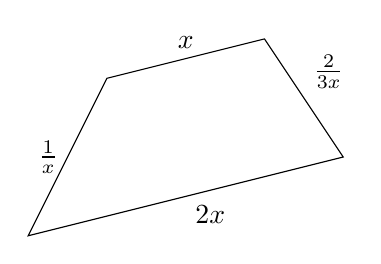
\begin{tikzpicture}[scale=1]
\draw (0,0) -- (4,1) node[midway, below right] {$2x$}
      -- (3,2.5) node[midway, above right] {$\frac{2}{3x}$}
      -- (1,2) node[midway, above] {$x$}
      -- cycle node[midway, left] {$\frac{1}{x}$};
\end{tikzpicture}
\end{center}
\answer{}
\end{practice}

\section*{PRACTICE \& PROBLEM SOLVING}
\textbf{UNDERSTAND}
\begin{practice}{12}{unknown}
\textbf{Generalize} Explain how addition and subtraction of rational expressions is similar to and different from addition and subtraction of rational numbers.
\answer{}
\end{practice}

\begin{practice}{13}{unknown}
\textbf{Error Analysis} Describe and correct the error a student made in adding the rational expressions.
\begin{align*}
\frac{1}{x^2 + 3x + 2} + \frac{x^2 + 4x}{4x + 8} &= \frac{1}{(x + 1)(x + 2)} + \frac{x(x + 4)}{4(x + 2)} \\
&= \frac{4}{4(x + 1)(x + 2)} + \frac{x(x + 4)}{4(x + 1)(x + 2)} \\
&= \frac{4 + x^2 + 4x}{4(x + 1)(x + 2)} \\
&= \frac{x^2 + 4x + 4}{4(x + 1)(x + 2)} \\
&= \frac{(x + 2)(x + 2)}{4(x + 1)(x + 2)} \\
&= \frac{x + 2}{4(x + 1)} \cdot \frac{(x + 2)}{(x + 2)} \\
&= \frac{x + 2}{4(x + 1)} \quad {\color{red} \boldsymbol{\times}}
\end{align*}
\answer{}
\end{practice}

\begin{practice}{14}{unknown}
\textbf{Use Structure} Find the slope of the line that passes through the points shown. Express in simplest form.
\begin{center}
\begin{tikzpicture}[scale=0.8]
\draw[<->] (-5,0) -- (5,0) node[right] {$x$};
\draw[<->] (0,-3) -- (0,5) node[above] {$y$};
\foreach \x in {-4,-2,2,4} \draw (\x,0.1) -- (\x,-0.1) node[below] {\x};
\foreach \y in {-2,2,4} \draw (0.1,\y) -- (-0.1,\y) node[left] {\y};
\fill[red] (-1,-1) circle (2pt) node[below left, black] {$\left(-\frac{1}{b}, -\frac{1}{a}\right)$};
\fill[red] (2,0.5) circle (2pt) node[above right, black] {$\left(2, \frac{1}{b}\right)$};
\draw[thick, <->] (-3,-1.5) -- (4,1);
\end{tikzpicture}
\end{center}
\answer{}
\end{practice}

\begin{practice}{15}{unknown}
\textbf{Reason} For what values of $x$ is the sum of $\frac{x - 5y}{x + y}$ and $\frac{x + 7y}{x + y}$ undefined? Explain.
\answer{}
\end{practice}

\begin{practice}{16}{unknown}
\textbf{Look for Relationships} Find the LCM of $3x^2 + 7x + 2$ and $9x + 3$.
\answer{}
\end{practice}

\begin{practice}{17}{unknown}
\textbf{Higher Order Thinking} Why are rational expressions closed under addition?
\answer{}
\end{practice}

\textbf{PRACTICE}
\textbf{Find the sum.} SEE EXAMPLE 1
\begin{practice}{18}{unknown}
$\frac{4x}{x + 7} + \frac{9}{x + 7}$
\answer{}
\end{practice}
\begin{practice}{19}{unknown}
$\frac{3y - 1}{y^2 + 4y} + \frac{9y + 6}{y(y + 4)}$
\answer{}
\end{practice}

\textbf{Find the LCM for each group of expressions.} SEE EXAMPLE 2
\begin{practice}{20}{unknown}
$x^2 - 7x + 6, x^2 - 5x - 6$
\answer{}
\end{practice}
\begin{practice}{21}{unknown}
$y^2 + 2y - 24, y^2 - 16, 2y$
\answer{}
\end{practice}

\textbf{Find the sum.} SEE EXAMPLE 3
\begin{practice}{22}{unknown}
$\frac{6x}{x^2 - 8x} + \frac{4}{2x - 16}$
\answer{}
\end{practice}
\begin{practice}{23}{unknown}
$\frac{3y}{2y^2 - y} + \frac{2}{2y}$
\answer{}
\end{practice}

\textbf{Find the difference.} SEE EXAMPLE 4
\begin{practice}{24}{unknown}
$\frac{4x}{x^2 - 1} - \frac{4}{x - 1}$
\answer{}
\end{practice}
\begin{practice}{25}{unknown}
$\frac{y - 1}{3y + 15} - \frac{y + 3}{5y + 25}$
\answer{}
\end{practice}

\begin{practice}{26}{unknown}
On Saturday morning, Ahmed decided to take a bike ride from one end of the 15-mile bike trail to the other end of the bike trail and back. His average speed the first half of the ride was 2 mph faster than his speed on the second half. Find an expression for Ahmed's total travel time. If his average speed for the first half of the ride was 12 mph, how long was Ahmed's bike ride? SEE EXAMPLE 5

\placeholder{illustration}{A person riding a bicycle on a trail. Labels: Speed x+2, Trail length 15 miles, Speed x}
\answer{}
\end{practice}

\textbf{Write each expression in its simplest form.} SEE EXAMPLE 6
\begin{practice}{27}{unknown}
$\frac{1 + \frac{1}{x}}{x - \frac{1}{x}}$
\answer{}
\end{practice}
\begin{practice}{28}{unknown}
$\frac{\frac{3}{y} + \frac{7}{x}}{\frac{1}{y} - \frac{2}{x}}$
\answer{}
\end{practice}
\begin{practice}{29}{unknown}
$\frac{\frac{1}{a} + \frac{1}{b}}{\frac{a^2 - b^2}{ab}}$
\answer{}
\end{practice}
\begin{practice}{30}{unknown}
$\frac{\frac{z^2 - z - 12}{z^2 - 2z - 15}}{\frac{z^2 + 8z + 12}{z^2 - 5z - 14}}$
\answer{}
\end{practice}

\textbf{APPLY}
\begin{practice}{31}{unknown}
\textbf{Use Structure} Aisha paddles a kayak 5 miles downstream at a rate 3 mph faster than the river's current. She then travels 4 miles back upstream at a rate 1 mph slower than the river's current. Hint: Let $x$ represent the rate of the river current.

\placeholder{illustration}{A person paddling a kayak. Labels: Kayak's downstream speed is x+3 mph, Water current's speed is x mph}

\begin{enumerate}
    \item[\textbf{a.}] Write and simplify an expression to represent the total time it takes Aisha to paddle the kayak 5 miles downstream and 4 miles upstream.
    \item[\textbf{b.}] If the rate of the river current, $x$, is 2 mph, how long was Aisha's entire kayak trip?
\end{enumerate}
\answer{}
\end{practice}

\begin{practice}{32}{unknown}
\textbf{Model With Mathematics} The resistance of electrical circuits A and B are shown. Find the ratio of the resistance of Circuit A to Circuit B.
\begin{center}
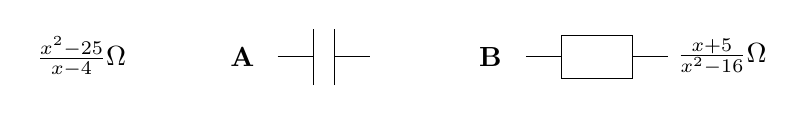
\begin{tikzpicture}[scale=0.9]
\node[left] at (0,0) {$\frac{x^2 - 25}{x - 4} \Omega$};
\node at (1.5,0) {\textbf{A}};
\draw (2,0) -- (2.5,0);
\draw (2.5,-0.4) -- (2.5,0.4);
\draw (2.8,-0.4) -- (2.8,0.4);
\draw (2.8,0) -- (3.3,0);

\begin{scope}[shift={(5,0)}]
\node at (0,0) {\textbf{B}};
\draw (0.5,0) -- (1,0);
\draw (1,-0.3) rectangle (2,0.3);
\draw (2,0) -- (2.5,0);
\node[right] at (2.5,0) {$\frac{x + 5}{x^2 - 16} \Omega$};
\end{scope}
\end{tikzpicture}
\end{center}
\answer{}
\end{practice}

\begin{practice}{33}{unknown}
\textbf{Reason} The Bello family drives 180 miles (round trip) to a professional basketball game. On the way to the game, their average speed is approximately 8 mph faster than their speed on the return trip home.
\begin{enumerate}
    \item[\textbf{a.}] Let $x$ represent their average speed on the way home. Write and simplify an expression to represent the total time it took them to drive to and from the game.
    \item[\textbf{b.}] If their average speed going to the game was 62 mph, how long did it take them to drive to the game and back?
\end{enumerate}
\answer{}
\end{practice}

\textbf{ASSESSMENT PRACTICE}
\begin{practice}{34}{unknown}
Which of the following compound fractions simplifies to $\frac{x + 1}{x - 3}$? Select all that apply.
\begin{itemize}
    \item[$\square$] $\frac{\frac{x^2 + 5x + 4}{x^2 + 2x - 8}}{\frac{x^2 - 4x + 3}{x^2 - 3x + 2}}$
    \item[$\square$] $\frac{\frac{x^2 - 1}{x^2 - 4}}{\frac{x^2 + x - 7}{x^2 + 5x + 6}}$
    \item[$\square$] $\frac{\frac{x^2 + 3x - 10}{x^2 - 16}}{\frac{x^2 - 4x - 5}{x^2 - 1}}$
    \item[$\square$] $\frac{\frac{x^2 + 3x - 10}{x^2 - 5x + 6}}{\frac{x^2 - 25}{x^2 - 4x - 5}}$
\end{itemize}
\answer{}
\end{practice}

\begin{practice}{35}{unknown}
\textbf{SAT/ACT} What is the difference between $\frac{x}{9}$ and $\frac{x - y}{6}$?
\begin{enumerate}
    \item[\textbf{A}] $\frac{5x - y}{18}$
    \item[\textbf{B}] $\frac{5x + y}{18}$
    \item[\textbf{C}] $\frac{-x + 3y}{18}$
    \item[\textbf{D}] $\frac{-x - 3y}{18}$
\end{enumerate}
\answer{}
\end{practice}

\begin{practice}{36}{unknown}
\textbf{Performance Task} The lens equation $\frac{1}{f} = \frac{1}{d_i} + \frac{1}{d_o}$ represents the relationship between $f$, the focal length of a camera lens, $d_i$, the distance from the lens to the film, and $d_o$, the distance from the lens to the object.

\placeholder{illustration}{Diagram of a camera lens focusing light from an object to an image screen. Labels: Object, f, f, d_o, d_i, Image screen, Lens}

\textbf{Part A} Find the focal length of a camera lens if an object that is 12 cm from a camera lens is in focus on the film when the lens is 6 cm from the film.

\textbf{Part B} Suppose the focal length of another camera lens is 3 inches, and the object to be photographed is 5 feet away. What distance (to the nearest tenth inch) should the lens be from the image screen?
\answer{}
\end{practice}

\end{document}